\documentclass[Main.tex]{subfiles}

\begin{document}
\section{Dataset}

Zoals reeds in de introductie aangehaald is er op het moment van schrijven geen bestaande dataset die geschikt is voor het onderzochte probleem. Aangezien het noodszakelijk is om voor de experimenteren, is er nood aan zelfgegenereerde datasets. Er zijn verschillende manieren om datasets te genereren. Het doel is de verwachte gebruikersdata zo goed mogelijk na te bootsen.
  
\subsection{Verschillende randomgeneratoren}
\subsubsection*{Volledig willekeurig}
Elke waarde die gegenereerd wordt, is een willekeurig getal tussen 0 en 100. Het voordeel aan deze generator is het feit dat geen enkel algoritme wordt bevoordeeld met de dataset. Een nadeel is echter het feit dat er weinig tot geen structuur zit in een willekeurige reeks van getallen, laat dat net hetgene zijn waar door het algoritme gezocht wordt. Bovendien wordt er verwacht dat er een zekere structuur zit in de gebruiker gedefinieerde data.

\subsubsection*{Gestructureerd}
Het doel van deze datasets is een willekeurige vergelijking te genereren waaraan vervolgens de data zal voldoen. Er wordt vanuit gegaan dat er \'e\'en constante gezocht wordt en dat elke kolomwaarde slechts \'e\'enmaal voorkomt. Voordelig hieraan is dat er altijd een oplossing bestaat, indien alle mogelijkheden van de boom ge\"evalueerd worden. Het feit dat er altijd een oplossing gevonden wordt, toont aan dat er een bepaald voordeel gegeven aan het geoptimaliseerde algoritme dat gebruikt maakt van gewichten.

\begin{center}
\begin{tabular}{@{} *5l @{}}    \toprule
\multicolumn{5}{l}{\emph{Volledig willekeurig}}\\\midrule
 Vergelijking & A  & B  & C  & D  \\ 
 Vgl 1. & 2 & 17 & 33 & 3\\ 
 Vgl 2. & 19 & 78 & 10 & 63\\\bottomrule
 \hline
\end{tabular}

\begin{tabular}{@{} *5l @{}}    \toprule
\multicolumn{5}{l}{\emph{Gestructureerd: } $B*C+C+A = D$} \\ \midrule
 Vergelijkingen & A  & B  & C  & D  \\ 
 Vgl 1. & 2 & 7 & 3 & 30\\ 
 Vgl 2. & 14 & 18 & 1 & 50\\\bottomrule
 \hline
\end{tabular}

\begin{tabular}{@{} *5l @{}}    \toprule
\multicolumn{5}{l}{\emph{Complex gestructureerd:}  $4*A+C*C$}\\\midrule
 Vergelijkingen & A  & B  & C  & D  \\ 
 Vgl 1. & 2 & 7 & 3 & 17\\ 
 Vgl 2. & 14 & 18 & 1 & 57\\\bottomrule
 \hline
\end{tabular}
\end{center}

\subsubsection*{Complex gestructureerd}
Deze datagenerator heeft als doel de gebruikersdata beter te benaderen. Dit wordt bereikt door randomfactoren toe te voegen aan de generator. Zo zal in deze generator er gekozen worden tussen een random aantal gewichten, liggend tussen nul en twee. Ook wordt het voorkomen van de kolomwaarden random bepaald. Zo is het mogelijk dat in de gezochte vergelijking een bepaalde kolomwaarde niet voorkomt en een andere meermaals.

\begin{figure}
\centering
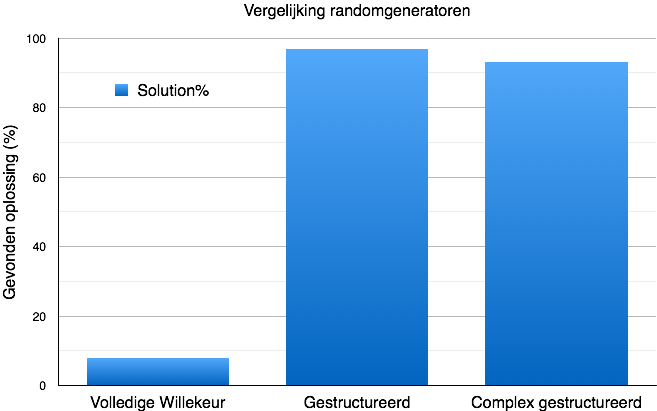
\includegraphics[width=\columnwidth]{compGene.png}
\caption{Vergelijking datageneratoren met gebruik van brute force algoritme} \label{fig:datageneratoren}
\end{figure}

\subsection{Verantwoording keuze}
Om de meest geschikte datagenerator te bepalen is er een vergelijking nodig tussen de datasets die gecre\"eerd worden. Er moet voldaan zijn aan het volgende criterium: de gegenereerde dataset ligt zo dicht mogelijk bij re\"ele gebruikersdata. De generatoren worden vergeleken met het brute force algoritme. Aangezien het geoptimaliseerd algoritme nooit vergelijkingen zal vinden die het brute force algoritme niet vindt, moet er een redelijke oplossingsgraad zijn met brute force algoritme. In figuur \ref{fig:datageneratoren} wordt de oplossingsgraad weergegeven. Hieruit blijkt dat de complex gestructureerde random generator het dichtst ligt bij de verwachte gebruikersdata. Daarom zullen de experimenten ook met behulp van deze generator worden uitgevoerd.

\end{document}